\chapter{Systembeskrivelse}
Det er under operationer vigtigt at benyttet et system, som er i stand til at måle patientens blodtryk. Dette gør det muligt for det tilstedeværende sundhedspersonale at danne sig et overblik, over patientens helbredstilstand. Blodtryksmåleapparaturet BTM er et sådan system. Som det ses på figur \ref{fig:Systemoversigt} består BTM af to snitflader, såkaldte interfaces, til omverdenen. En transducer opfanger blodtryk fra en patient, eller et væsketryk fra et kalibreringsudstyr og oversætter dette til et elektrisk signal, som BTM kan vise på sit indbyggede display. Dette signal lagres internt i BTM, som en datafil, der senere kan overføres til et filarkiv. Blodtryksmåleapparaturet BTM betjenes af sundhedspersonalet, ved brug af stemmekommadoer. 
\begin{figure}[htbp]
\centering
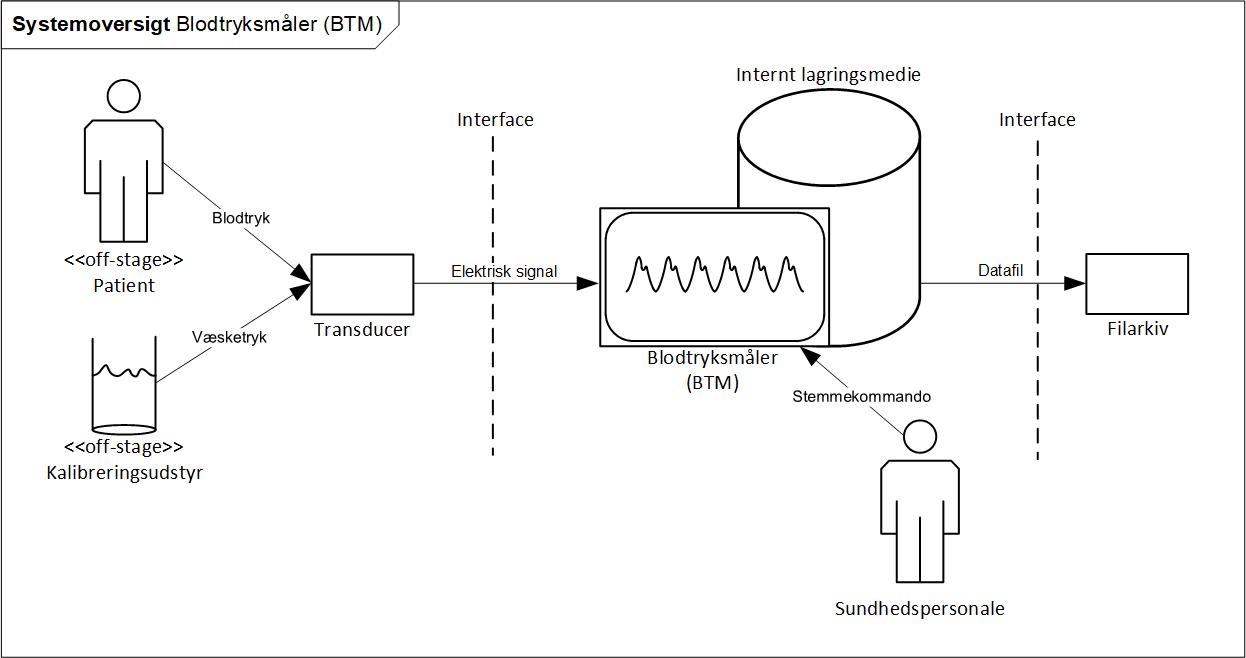
\includegraphics[width=1.00\textwidth]{billeder/Systemoversigt.png}
\caption{Systemoversigt over blodtryksmåleapparatur (BTM)}
\label{fig:Systemoversigt}
\end{figure}
